%----------------------------------------------------------------------------
\chapter{Introduction of SensorML and SensorWeb}\label{sect:Introduction}
%----------------------------------------------------------------------------
\section{Goals of observation gathering}
%----------------------------------------------------------------------------
Most phyisical quantities are measured with great accuracy on very basic devices. From the most basic sound measurements with microphone, to the nowadays popular inertial measurement units every data can be measured. There are also weather sensors and solar sensors available for everyone.

 With the evolution of sensor fusion algorithms these data can be merged together to give an even better accuracy or a general knowledge of our environment. This data can be used to predict weather conditions by merging neighborhood sensors into one. It can be used to make predictions based on the weather conditions in an area and the direction of the wind on the location.
 
 \begin{figure}[h]
 \centering
 %http://www.crystaldatainternational.com/choices/sensorml.html
  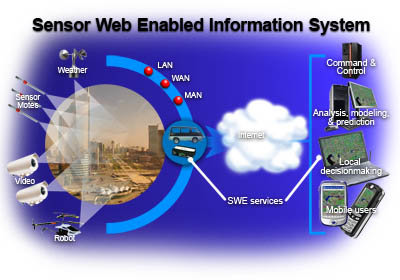
\includegraphics[width=0.6\textwidth]{figures/webswe.png}
 \caption{SWE architecture\label{fig:webswe}}
 \end{figure}
 
 
 The other challenge is to use a sensor's data for multiple purposes. For example a CCTV camera picture can be used to count the number of cars on the road, to get an estimation of the speedings in a crossing or to get visual weather data. Computer Vision algorithms, regressions and special machine learning algorithms need different computing resources. Those can be outsourced to different computers which must have access to the data. The Sensor Observation Server is used to make this all available.
 
 \section{Types of sensors}
 
 Sensors are all around us. We have sensors in our cell phones or any handheld devices. Most of them are connected to the internet or a network. The measurements of all of these devices can be stored and queried from a database. The usable data in some devices are:
 
 \begin{itemize}
 	\item Smartphone
 	 \begin{itemize}
	 	 \item Camera: Visual image of the phone itself
	 	 \item Accelerometer: measurement of the acceleration of a system. Derivate of speed.
	 	 \item Weather sensors: Often smartphones has built in temperature sensors, rarely barometer is also installed.
	 	 \item Computing resource: ability to run additional softwares by using up its resources
	 	 \item Gyroscope: Orientation sensor.
 	 \end{itemize}
 	 \item Weather sensor
 	 \begin{itemize}
 	 \item Tempareture sensor: Inner and outer temperature.
 	 \item Humidity sensor: percentage of humidity.
 	 \item Barometer: Air pressure.
 	 \end{itemize}
 	 \item Beagleboard
 	 \begin{itemize}
	\item Computing resource.
 	 \end{itemize}
 \end{itemize}

The examples show that a standard way to retrieve the measurements should include not only the measurement, but the type of the sensor, the measured unit, the location of the sensor and many additional information like this. This is done using the SensorML.

\section{The SensorML}

The Open Geospatial Consortium approved the SensorML language to be able to describe all the necessary information about measured data\cite{sensorml}. This is an XML based language that is used to describe the sensors, add, update, delete or retrieve information. The SensorML is able to solve the above mentioned problems. It is an abstract definition of the sensor information.
It is able to define the location of the sensor, the timestamp of the measurement and the sensor data itself, with many additional information. The data can be stored in SOS servers that can retrieve the data on different interfaces.
 
\section{Server Observation Service}

Server Observation Servers store SensorML data and let others query, manipulate and add sensors to the database. These sensors can be derived sensors. Such derived sensors are called procedures. A procedure can be a traffic information based on the CCTV camera. An SOS server should be able to handle dependencies based on which procedure requires other procedures to provide data. Sometimes derived sensors are also called virtual sensors, because they don't do physical measurement but provide a derived value.

There are many closed and open source implementations of SOS servers. Some open source implementations are introduced here.

The MapServer is written in C, C++, however it can be extended in many other languages\cite{mapserver}. It has a built in GUI to view data, however it is not yet available for the SOS implementation. The server can only be reached by one interface. It was originally developed by University of Minnesota. In the time of writing the paper the code is maintained and supported by the Open Source Geospatial Foundation. It is mostly used for mapping not for serving data for derived sensors. It was used in some projects between NASA and the University of Minnesota. 

istSOS is another implementation in Python\cite{istsos}. It runs its scripts from Apache web server just like MapServer. It uses PostgreSQL database backend to store values. It has a nice GUI for administration. Only supports standard SensorML interface to retrieve data. It is a project of the SUPSI University in Switzerland.

OOSThetys is a basic toolkit for enabling SensorML communication. It is written in Perl and Java. It is fairly documentated and seems to be abandoned because there has been no new release since the February of 2012.

52north SOS is a sample implementation written in Java\cite{52north}. It runs as a web service from Apache tomcat to serve requests. It also uses PostgreSQL with PostGIS extension. The application is used in the sample implementation and it is covered in details later.

All SOS servers and the whole SensorML standard is missing the semantic information about the sensors meaning that all sensor data are stored in such a database and all properties can be described for the sensors but no connection between the concepts can be described for the sensor.

\section{52north SOS server}

This implementation is done by the non profit organization with the identical name. The software supports many interfaces to query the information needed. The standard SOAP can be used to work with Java Web services. There are KVP and POX to retrieve or add data using standard GET queries. A big advantage is that 52north SOS supports JSON interface. It enables RESTful JSON queries to retrieve information efficiently in JavaScript, PHP, Python or other modern scripting languages.

The new 4.2 version is easy to install, it has a graphical user interface to set up the database connection and initialize the database. PostgreSQL with PostGIS is required.  The basic usage is described on  52north webpage, but sample queries are shown in the built in test client. 

The project is built with Maven and uses Spring framework too. The included unit tests ensure that the software's architecture is still consistent after compilation. The project was chosen to be part of Google's Summer of Code 2014 and the project gained a lot improvements from that. 

A request can be sent using the connector of each interface. This used to be done by adding the interface name to the application url but in recent versions the service automatically detects the interface from the HTTP metadata. For example http://152.66.253.152:8080/52n-sos-webapp/service is the url where all interface can be reached. The first part is the host of the server. The tomcat application server is listening on port 8080. 52n-sos-webapp is the default name of the web application, service it the default connector for the webservice. The sent HTTP content-type header marks the interface. For example application/json stands for the JSON and application/soap+xml stands for SOAP interface.

\section{SOS commands}
There are many commands to query or manipulate the SOS server. There are only two important commands that should be described in details. These are GetCapabilities and GetObservations.

GetCapabilities command allows the clients to retrieve a list of the reachable sensors of the server and their configuration. This call does not have any required parameters, only if the details of the response should be controlled.

\begin{lstlisting}[caption={JSON getCapabilities POST request\label{lst:getcap}}]
{
  "request": "GetCapabilities",
  "service": "SOS",
  "sections": [
    "Contents"
  ]
}
\end{lstlisting}

The GetObservation retrieves the stored measurements. The timerange and the procedure (sensor) id shall be specified. The answer differs on each interfaces, but data is usually given as ASCII characters separated by previously specified markers.

\begin{lstlisting}[caption={SOAP getObservationById POST request\label{lst:getobs}}]
<?xml version="1.0" encoding="UTF-8"?>
<env:Envelope
    xmlns:env="http://www.w3.org/2003/05/soap-envelope"
    xmlns:xsi="http://www.w3.org/2001/XMLSchema-instance"
     xsi:schemaLocation="http://www.w3.org/2003/05/soap-envelope
      http://www.w3.org/2003/05/soap-envelope/soap-envelope.xsd">
    <env:Body>
        <sos:GetObservationById
            xmlns:sos="http://www.opengis.net/sos/2.0"
             service="SOS" version="2.0.0"
              xsi:schemaLocation="http://www.opengis.net/sos/2.0
               http://schemas.opengis.net/sos/2.0/sos.xsd">
            <sos:observation>
            http://www.52north.org/test/observation/1
            </sos:observation>
            <sos:observation>
            http://www.52north.org/test/observation/2
            </sos:observation>
        </sos:GetObservationById>
    </env:Body>
</env:Envelope>
\end{lstlisting}
Such commands are used by the client softwares to display information.

\section{SOS client applications}

52north has a client application for the SOS server called 52n Sensorweb Client. This is a Java web application that can be configured to connect to multiple hosts and display their sensor data on maps and charts. It is developed using the same tools as the SOS server. This client is a web application which is can be opened in a web browser, but some parts run on the web server. This is a relatively complex application that does not yet understand semantic connections between the procedures. A screenshot can be seen on figure \ref{fig:sweclient}.

\begin{figure}[h]
\centering
%http://sensorweb.forum.52north.org/SWE-Client-Could-not-get-procedure-details-url-caused-by-java-lang-NullPointerException-td4025524.html
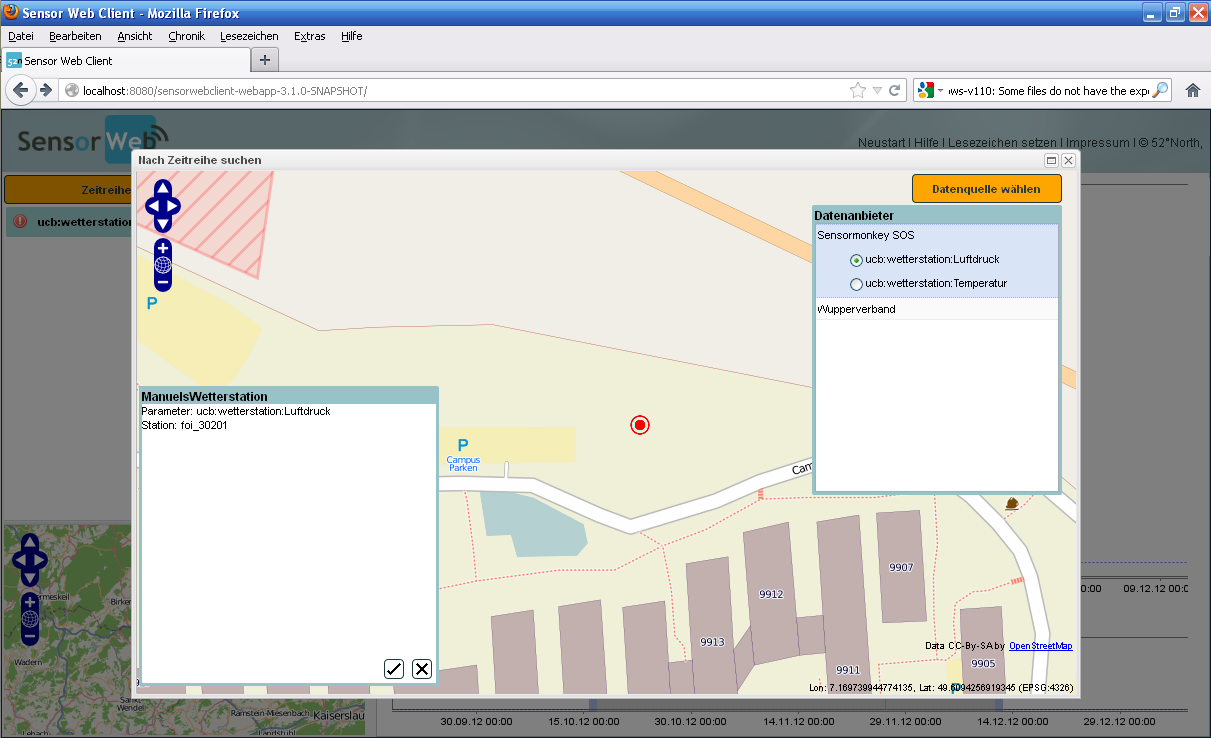
\includegraphics[width=0.6\textwidth]{figures/sweclient.png}
\caption{Screenshot of SWE Client 3\label{fig:sweclient}}
\end{figure}

There is a JavaScript framework that enables users to use only client side tools to connect to SOS servers and display data called SOS.js. Unfortunately, because of security restrictions on JavaScript cross-site request the data cannot be retrieved from the SOS server directly, the client has to be served from the same domain as the server. This is often not doable. That is why this application needs a proxy that forwards the data to the same domain to bypass this restriction. Screenshot can be seen on figure \ref{fig:sos-js}.

\begin{figure}[h]
\centering
%http://blog.52north.org/2014/02/21/sos-js/
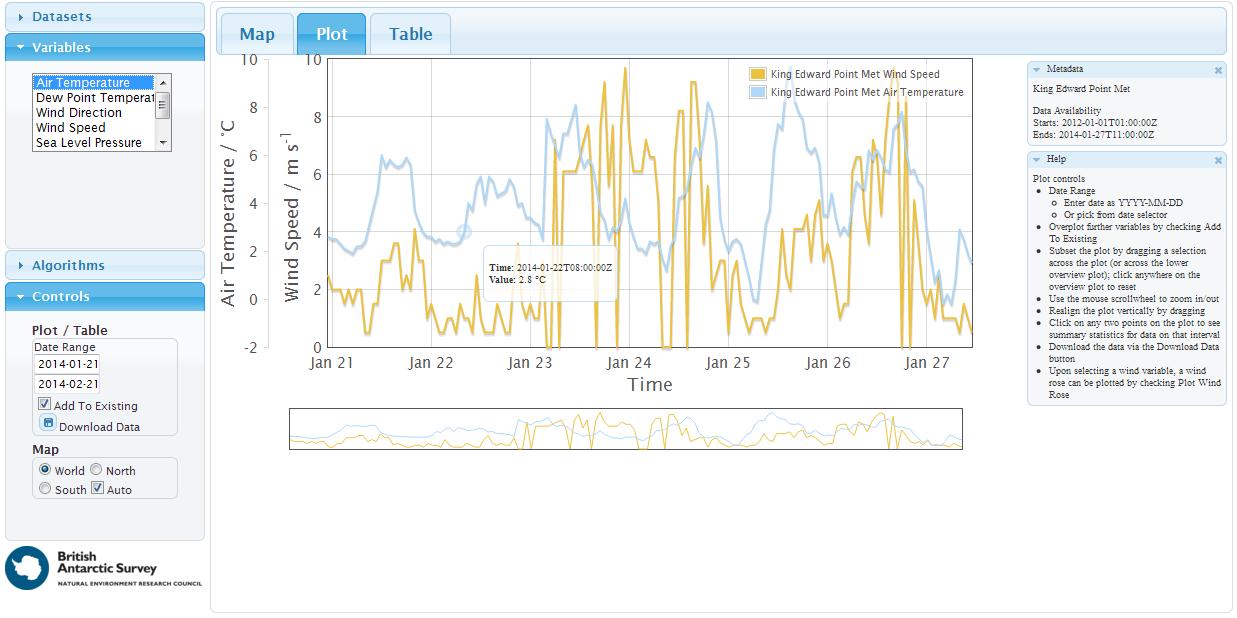
\includegraphics[width=0.6\textwidth]{figures/sos-js.png}
\caption{Screenshot of sos.js\label{fig:sos-js}}
\end{figure}

There are external softwares that can display their own measurements but not the SensorML standard. To make them usable with 52north SOS the developers created tools to extend such existing softwares to be able to import data from SOS. Such extension is the ArcGIS extension which makes SOS data available to ArcGIS server. This is also available to other programs such as $\mu$Dig. 

There are other tools to export data to R language or to use with other Geographic Information Systems (GIS) softwares. However, the problem is that no client software has the ability to make search available by semantic connections. A client has to be extended with such information to enable convenient filtering when monitoring a cyberphisical system.


